\subsection{Quicksort a Tre Partizioni}
\texttt{Quicksort} con \texttt{RandomizedPartition} funziona bene ed 
evita, quasi in ogni circostanza, di imbattersi nel caso pessimo, ad 
eccezione di un caso particolare: se in \emph{input} viene dato un 
array con tutti gli elementi uguali, si ottiene il temuto caso pessimo $O(n^2)$.\par
Per ovviare al problema, è sufficiente partizionare \texttt{Quicksort} in tre
partizioni invece di due. Dato un \emph{pivot} $x$, partizioniamo $A$ nel
seguente modo:

\begin{center}
    \begin{tabular}{|l|l|l|}
        \hline 
        $< x$ & $= x$ & $> x$ \\
        \hline
    \end{tabular}
\end{center}

Durante l'algoritmo, la disposizione sarà questa:

\begin{center}
    \begin{tabular}{|l|l|l|l|}
        \hline 
        $< x$ & $= x$ & $\quad$ & $> x$ \\
        \hline
    \end{tabular}
\end{center}
(La cella vuota è la regione ancora da esplorare).

\begin{codebox}
\Procname{$\proc{Tripartition}(A,p,r)$}
\li $x \gets A[r]$
\li $i \gets p-1$
\li $k \gets p$
\li $j \gets r$
\li \While $k < j$
\li \Do
        \If $A[k] < x$
\li     \Then
        	$i \gets  i + 1$
\li         $A[i] \leftrightarrow A[k]$
\li         $k \gets k + 1$
\li		\ElseIf $A[k] > x$
\li		\Then
         	$j \gets j - 1$
\li         $A[j] \Leftrightarrow A[k]$
\li		\ElseNoIf
\li			$k \gets k + 1$
		\End
    \End
\zi \Comment $k = j$
\li $A[j] \Leftrightarrow A[r]$
\li \Return $(i+1,j)$ \Comment restituisce una coppia di valori
\end{codebox} 

\begin{codebox}
\Procname{$\proc{Quicksort}(A,p,r)$}
\li \If $p < r$
\li	\Then
		$\id{q_1},\id{q_2} \gets \proc{Tripartition}(A,p,r)$
\li		$\proc{Quicksort}(A,p,\id{q_1}-1)$
\li		$\proc{Quicksort}(A,\id{q_2}+1,r)$
	\End
\end{codebox} 

\subsection{Limite Inferiore}

\begin{itemize}[label=]
    \item \texttt{Input}: $a_1 \dots a_n$
    \item \texttt{Output}: permutazione $a'_1 \dots a'_n$ tale che
    $$a'_1 \leq a'_2 \leq \dots \leq a'_n$$
\end{itemize}

\paragraph{Confronti e assegnamenti} 

Osservazioni:
\begin{itemize}[label=$\rightarrow$]
    \item Se ``conto'' solo alcune operazioni il limite inferiore
    vale in generale. Consideriamo solo l'operatore di confronto;
    \item Elementi tutti distinti $(a_i \neq a_j \text{ se } i \neq j)$,
    l'operatore di confronto $==$ restituisce sempre $\const{False}$.
\end{itemize}

\subsection{Albero di Decisione}

È una rappresentazione ``astratta'' delle possibili esecuzioni di un 
algoritmo di ordinamento su un input di dimensione fissata $A[1 \dots n]$.

\begin{itemize}[label=$\rightarrow$]
    \item nodi interni: 
    $$i \ : \ j \Rightarrow \text{confronta } A[i] \leq A[j]$$
    \item \emph{foglie} (ogni foglia è una possibile permutazione)
\end{itemize}

Ecco un esempio di \emph{Albero di Decisione} per l'array $A[a_1,a_2,a_3]$ 
con 
$$a_1 = 1, \; a_2 = 2, \; a_3 = 3$$
\clearpage
\begin{figure} 
    \centering
    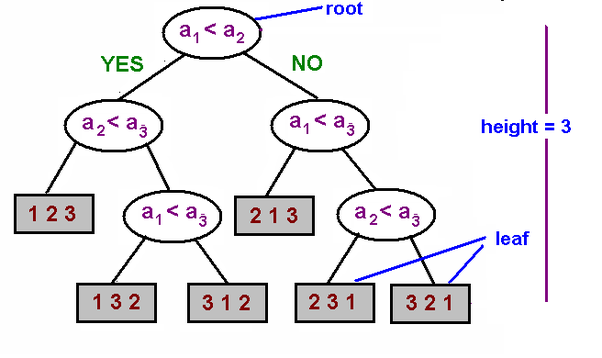
\includegraphics[width=\textwidth]{img/decision-tree.png}
    \caption{Albero di decisione per l'array $A[1,2,3]$}
\end{figure}

\paragraph{Osservazione}
\begin{itemize}
	\item $ \text{Altezza dell'albero di decisione} = \text{limite inferiore per caso pessimo}$
	\begin{align*}
	    \text{per }& \text{IS} \ \quad n^2 \\
	    \text{per }& \text{MS} \quad n \log n
	\end{align*}
	\item Ogni foglia ha una sola permutazione. Ogni permutazione compare (almeno) in una foglia.
\end{itemize}

\emph{In generale}, le foglie contengono \underline{tutte} le permutazioni.
$$ \text{\# foglie} \geq \text{\# permutazioni} = n! \qquad ( \text{\# foglie} \leq 2^h)$$
\begin{align*}
    h & \geq \log_2 n! \\
    & \geq \log_2 \left( n(n-1)(n-2) \dots \frac{n}{2}\right) \\
    & \geq \log_2 \left( \frac{n}{2}\left(\frac{n}{2}-1\right)\left(\frac{n}{2}-2\right) \dots \frac{n}{2}\right) \\
    & \geq \log_2 \left( \frac{n}{2} \right)^{(\frac{n}{2})} 
        = \frac{n}{2} \left( \log_2 n - \log_22\right)
        = \frac{n}{2} (\log_2 n - 1) = \Theta (n \log n)
\end{align*}
Inoltre,
\begin{itemize}
	\item $ \text{\# operazioni} \geq h = \Omega (n \log n)$
	\item $ \texttt{Heapsort, MergeSort } O(n \log n))$ 
\end{itemize}
$\Rightarrow \text{ordinamento (bastato su confronti) } \Theta (n \log n)$

\subsection{Counting Sort}
Esistono degli algoritmi di ordinamento che, in certe condizioni e per certi input, permettono
di ordinare in tempo lineare $\Omega (n)$
\bigskip

Assumo
\begin{itemize}[label=$-$]
    \item interi;
    \item in $[0,k]$
\end{itemize}

\begin{itemize}[label=]
    \item \texttt{Input}: $A[1\twodots n]$ con $A[j] \in [0,k] \quad \forall 1 \leq j \leq n$;
    \item \texttt{Output}: $B[1\twodots n]$ permutazione ordinata di $A$;
    \item \texttt{Supporto}: $C[0\twodots k]$.
\end{itemize}

\begin{codebox}
\Procname{$\proc{Counting-Sort}(A,B,k)$}
\li $C[0\twodots k] \leftarrow 0$
\li \For $j \gets 1$ \To $\attrib{A}{length}$
\zi \Do
		\Comment $C[x] =$ \verb|#| elementi in $A$ con valore $x$
\li		$C[A[j]] \gets C[A[j]] + 1$ 
    \End
\li \For $i \gets 1$ \To $k$
\zi \Do
        \Comment $C[x] =$ \verb|#| elementi in $A$ con valore $\leq x$
\li     $C[i] \gets C[i-1] + C[i]$ 
    \End
\li \For $j \gets \attrib{A}{length}$ \Downto $1$
\li \Do
        $B[C[A[j]]] \gets A[j]$
\li     $C[A[j]] \gets C[A[j]] - 1$
    \End
\end{codebox} 

\paragraph{Complessità} 
\begin{align*}
    C[0,k] \leftarrow 0 && \Theta(k) \\
    \text{\texttt{for j=1}} \dots && \Theta(n) \\
    \text{\texttt{for i=1}} \dots && \Theta(k) \\
    \text{\texttt{for j=A.length}} \dots && \Theta(n)
\end{align*}
$$\text{Somma } \Theta(n+k) \text{ con } k = \Theta(1) \Rightarrow \Theta(n)$$

\paragraph{Problema di memoria} Il problema di \texttt{CountingSort} è la memoria. 
Infatti, al crescere di $k$, la memoria richiesta per allocare \texttt{C} cresce esponenzialmente.
\begin{center}
    \begin{tabular}{|l|l|}
        \hline
        Dimensione $k$ & Memoria occupata da \texttt{C[]} \\
        \hline
        1 Byte $= 8$ bit & $2^8 \text{Bytes} = 256 \text{Bytes}$ \\
        2 Bytes $= 16$ bit & $2^{16} \text{Byte} \cdot 2 \text{Bytes} = 256 \text{Megabytes}$ \\
        8 Bytes $= 64$ bit & $2^{64} \text{Byte} \cdot 8 \text{Bytes} = 512 \text{Terabytes}$ \\
        \hline
    \end{tabular}
\end{center}

\subsubsection{Proprietà di Stabilità}
Dato $A[1 \twodots n]$ in input, se $A[i] \leq A[j]$ con $i \leq j$, allora nell'output $A[i]$ e $A[j]$ sono nello stesso ordine relativo.
\bigskip

Algoritmi stabili:
\begin{itemize}
	\item \texttt{MergeSort}
	\item \texttt{InsertionSort}
\end{itemize}
\bigskip

Algoritmi non stabili:
\begin{itemize}
	\item \texttt{CountingSort}
	\item \texttt{Quicksort}
	\item \texttt{Heapsort}
\end{itemize}